\section{Prompt Template}
\subsection{Prompt Template for Cold-Start Data Distillation}
\label{ap:distillation-template}
We show the template for cold-start data distillaion in Figure~\ref{fig:distialltion-template}.

\begin{figure*}[htbp]
  \centering
  % Row 1
  \begin{minipage}[t]{0.9\textwidth}
    \centering
    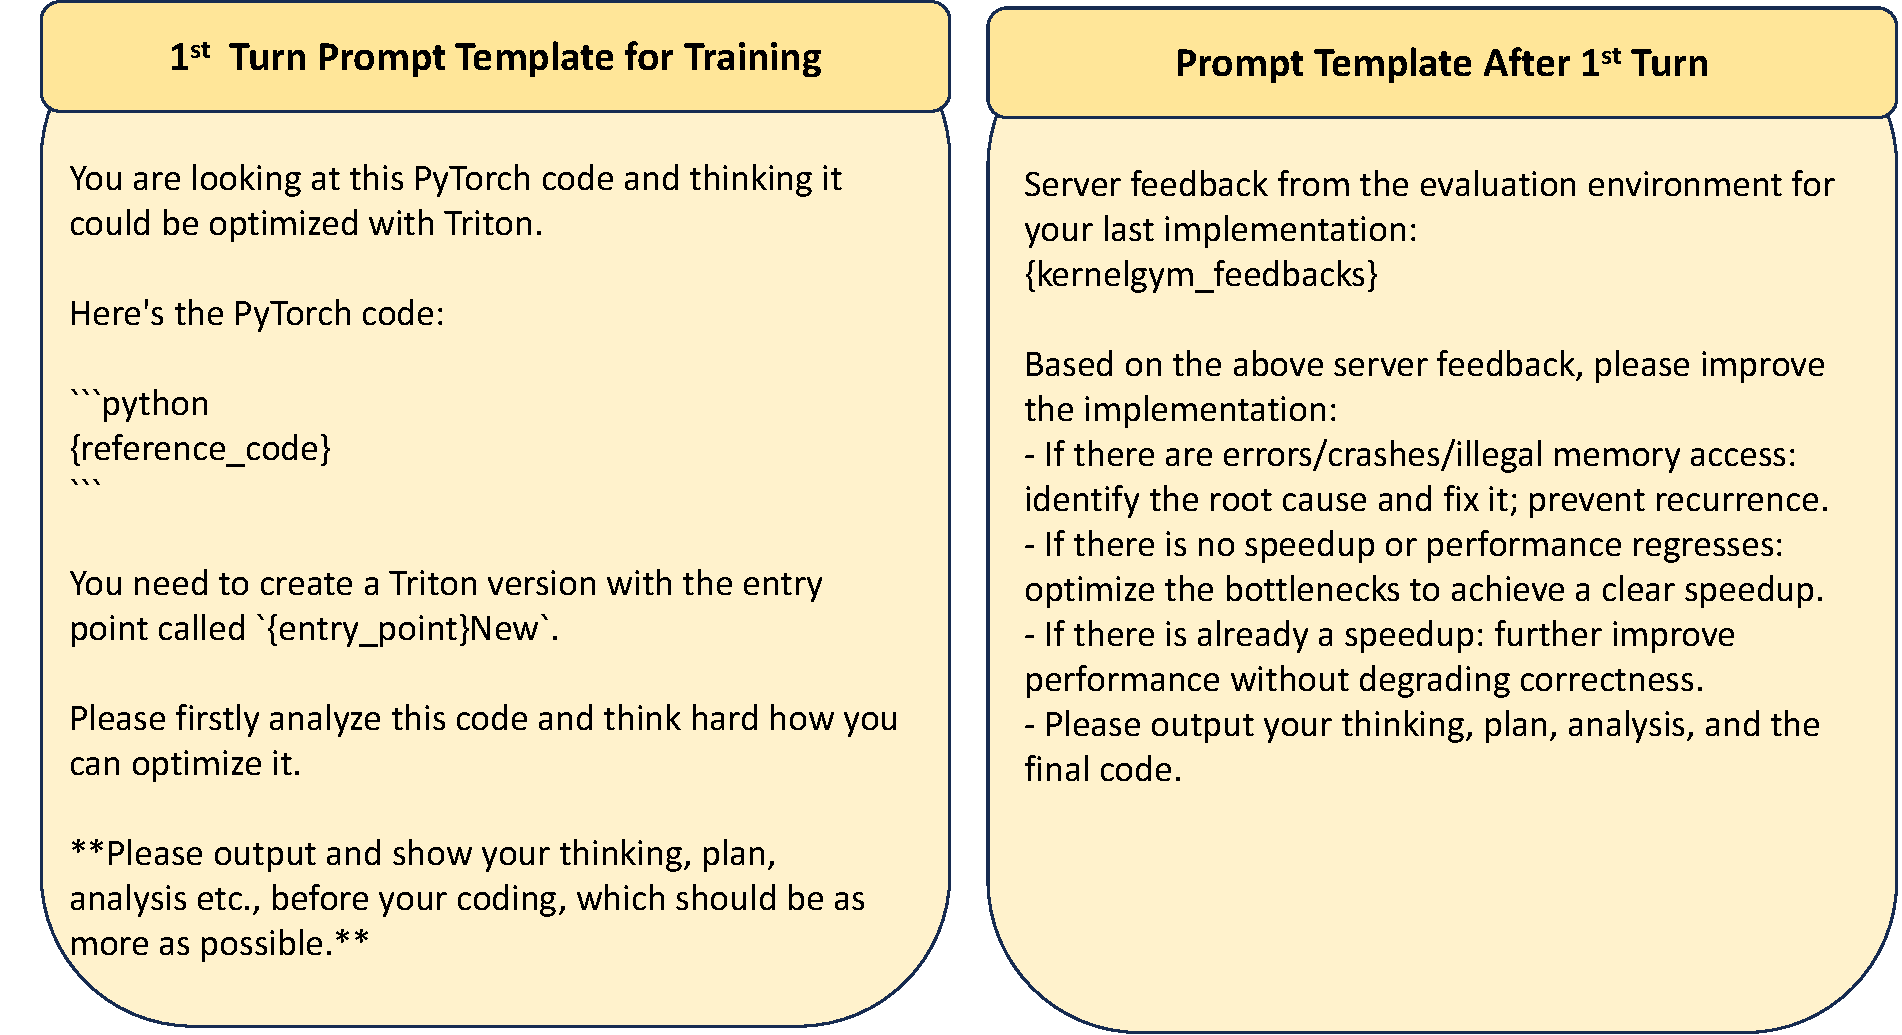
\includegraphics[width=\linewidth]{figures/prompt_template/distaillation_template.pdf}
  \end{minipage}
  \caption{The prompt template for cold-start data distillation.}
  \label{fig:distialltion-template}
\end{figure*}

\subsection{Prompt Template for SFT and RL}
We show the template for both SFT and RL in Figure~\ref{fig:training-template}.
\begin{figure*}[htbp]
  \centering
  % Row 1
  \begin{minipage}[t]{0.9\textwidth}
    \centering
    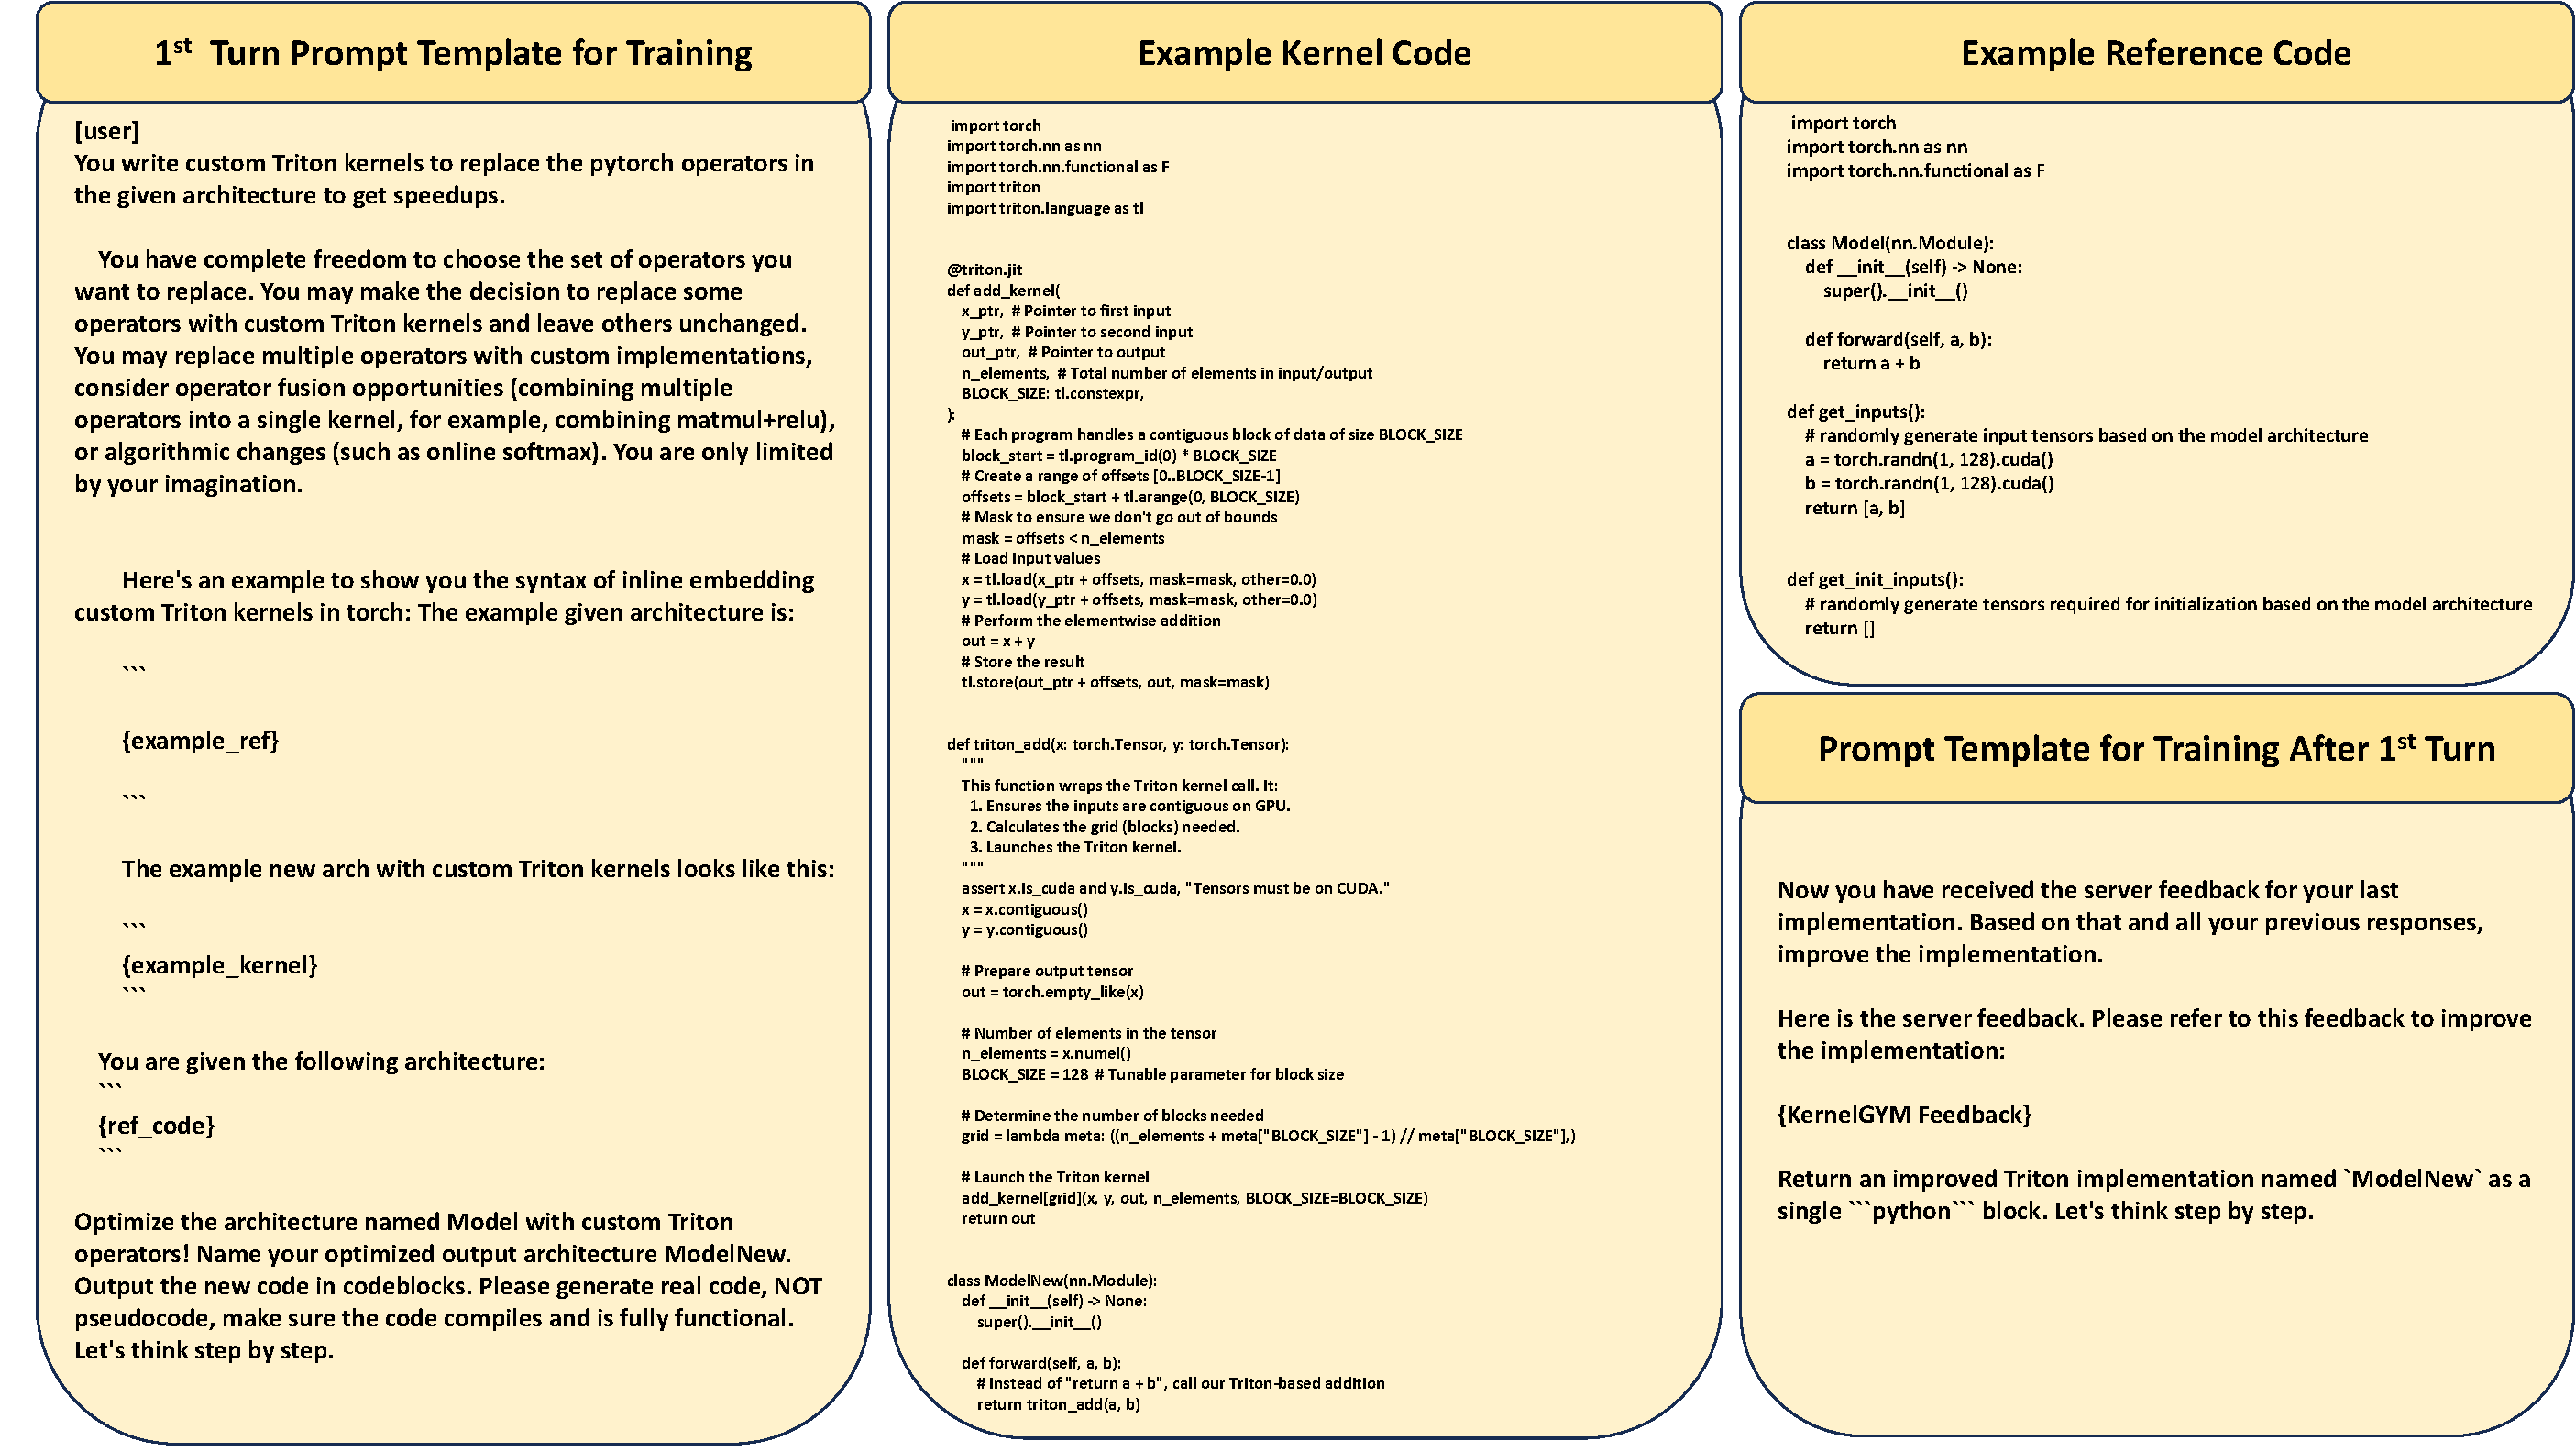
\includegraphics[width=\linewidth]{figures/prompt_template/training_prompt.pdf}
  \end{minipage}

  \caption{The prompt template for both SFT and RL. The task instruction, example code and reference code are shown in the first-turn prompt. And for the later turns, prompt asks model to refine the kernel implementaion based on all hisotory information and \env{} feedbacks.}
  \label{fig:training-template}
\end{figure*}